\documentclass{beamer}

\newcommand{\cmd}[1]{\textbf{\texttt{#1}}}
\newcommand{\pkg}[1]{\texttt{#1}}
\newcommand{\env}[1]{\texttt{#1}}
\newcommand{\opt}[1]{\textsl{#1}}

\usepackage{beamerthemesplit}
\beamertemplatenavigationsymbolsempty
\setbeamertemplate{footline}[page number]{}

\usepackage{graphicx}
\usepackage{color}
\usepackage{listings}
\usepackage{verbatim}
\usepackage{setspace}
\usepackage{url}

\usepackage{fontspec}
\setmonofont{Latin Modern Mono}
\setsansfont{TeX Gyre Heros}

\lstset{breakatwhitespace=true,
language=C++,
basicstyle=\footnotesize\ttfamily,
keywordstyle=\color{blue}\ttfamily,
stringstyle=\color{red}\ttfamily,
commentstyle=\color{brown}\ttfamily,
morecomment=[l][\color{magenta}]{\#}keepspaces=true,
breaklines=true,
tabsize=3,
showstringspaces=false,
extendedchars=true,
frame=single}

\newcommand*{\vcenteredhbox}[1]{\begingroup
\setbox0=\hbox{#1}\parbox{\wd0}{\box0}\endgroup}


\title{Building and Using the Bio-Formats C++ Implementation}
\author{Roger Leigh}
\date{Juin 2015\\Institut Pasteur}

\begin{document}

\begin{frame}[plain]
  \titlepage
  \begin{center}
    \vcenteredhbox{
\includegraphics[width=0.25\textwidth]{ome}} \hfill
    \vcenteredhbox{
\includegraphics[width=0.2\textwidth]{dundee}}\hfill
    \vcenteredhbox{
\includegraphics[width=0.25\textwidth]{wellcome}}
  \end{center}
\end{frame}

\section[]{Overview}
\frame{
\frametitle{Overview}
\tableofcontents
}

\begin{frame}
  \frametitle{Java and C++}
  \begin{itemize}
  \item \cmd{bf-itk-pipe} (pipe from C++ to JVM)
  \item \cmd{JACE} (wrap all Java classes, embed JVM)
  \item Bio-Formats-C++ (native C++ implementation)
    \pause
    \begin{itemize}
    \item Reference C++ OME-TIFF implementation
    \item OME-XML model objects
    \item Metadata store
    \item Reading
    \item Writing
    \end{itemize}
    \pause
  \item Initial uses:
    \begin{itemize}
    \item Image acquisition writing OME-TIFF
    \item Image analysis reading OME-TIFF
    \end{itemize}
  \end{itemize}
\end{frame}

\section{Prerequisites}
\subsection{Compiler and toolchain}

\begin{frame}
  \frametitle{Default compilers}
  \begin{itemize}
  \item FreeBSD: LLVM/\cmd{clang++} or GCC/\cmd{g++}
  \item Linux: GCC/\cmd{g++} and GNU Binutils/\cmd{ld}
  \item MacOS X: XCode (custom LLVM/\cmd{clang++})
  \item Windows: Visual Studio or Visual Studio Express (MSVC/\cmd{cl})
  \end{itemize}
\end{frame}

\subsection{Package installation}
\begin{frame}
  \frametitle{Package managers}
  \begin{itemize}
  \item FreeBSD: Ports (e.g. \cmd{pkg}, \cmd{portmaster})
  \item Linux: Distribution package manager (e.g. \cmd{apt-get} or \cmd{yum})
  \item MacOS X: homebrew (\cmd{brew})
  \item Windows: Yeah, right.  You need to manually download all the
    tools and then compile all the libraries by hand for your specific
    version of Visual Studio.  (Microsoft love to make development for
    their platform easy and painless.  Not!)
  \end{itemize}
\end{frame}

\begin{frame}
  \frametitle{Required packages}
  \scriptsize
  \begin{columns}
    \begin{column}{.5\linewidth}
      Libraries
      \begin{itemize}
      \item[] Boost
      \item[] HDF5
      \item[] PNG
      \item[] TIFF
      \item[] Xerces-C
      \end{itemize}
      \end{column}
    \begin{column}{.5\linewidth}
      Tools
      \begin{itemize}
      \item[] CMake
      \item[] Doxygen + Graphviz
      \item[] Git
      \item[] Graphicsmagick
      \item[] Python + genshi + sphinx
      \item[] \TeX{}Live
    \end{itemize}
    \end{column}
  \end{columns}
\end{frame}

\begin{frame}
  \frametitle{Windows installation (libraries)}

For python, either download separate installers for each packages, or
install \pkg{setuptools} and \pkg{pip} for Python, then \cmd{pip
  install} needed packages; ensure any downloaded packages are 64-bit
if using 64-bit python)
\bigskip

Build and install the following by hand (for Bio-Formats):
  \begin{columns}
    \begin{column}{.5\linewidth}
      \begin{itemize}
      \item[] \pkg{boost}
      \item[] \pkg{hdf5}
      \item[] \pkg{icu}
      \end{itemize}
    \end{column}
    \begin{column}{.5\linewidth}
      \begin{itemize}
      \item[] \pkg{tiff}
      \item[] \pkg{xerces}
      \item[] \pkg{zlib}
      \end{itemize}
    \end{column}
  \end{columns}
…and possibly more—we haven't yet done a Bio-Formats C++ build on Windows.
\end{frame}

\subsection{Configuration}

\begin{frame}
  \frametitle{System configuration}
  \begin{itemize}
    \item In general, none of the tools should require any configuration
      \item \LaTeX{} may require local font configuration to make the \TeX{} Gyre fonts available.
        \begin{itemize}
          \item Linux and FreeBSD: Use the provided \pkg{fontconfig}
            template or create your own
          \item MacOS X: Add to system using FontBook
          \item Windows: May need adding to the system fonts if not
            found automatically
        \end{itemize}
  \end{itemize}
\end{frame}

\begin{frame}
  \frametitle{Environment configuration}
  \begin{itemize}
    \item Primarily needed on Windows
    \item Rather than setting globally, make a batch file which can set up the environment.
    \item Activate a python virtualenv if needed
    \item Ensure that all tools are on the user \texttt{PATH}
      \begin{itemize}
        \item \cmd{cmake}, \cmd{doxygen}, \cmd{dot}, \cmd{git}, \cmd{python}, \cmd{sphinx}, \cmd{xelatex}
      \end{itemize}
    \item Set \texttt{CMAKE\_PREFIX\_PATH} if some libraries and tools are not on the default search path.
    \item Not all tools need to be on the default path; some will be discovered automatically by \cmd{cmake}
    \item No need to use a special Visual Studio shell when using \cmd{cmake}
  \end{itemize}
\end{frame}

\section{Building Bio-Formats}

\subsection{cmake introduction}

\begin{frame}
  \frametitle{\cmd{cmake} overview}
  \medskip
  \centering
  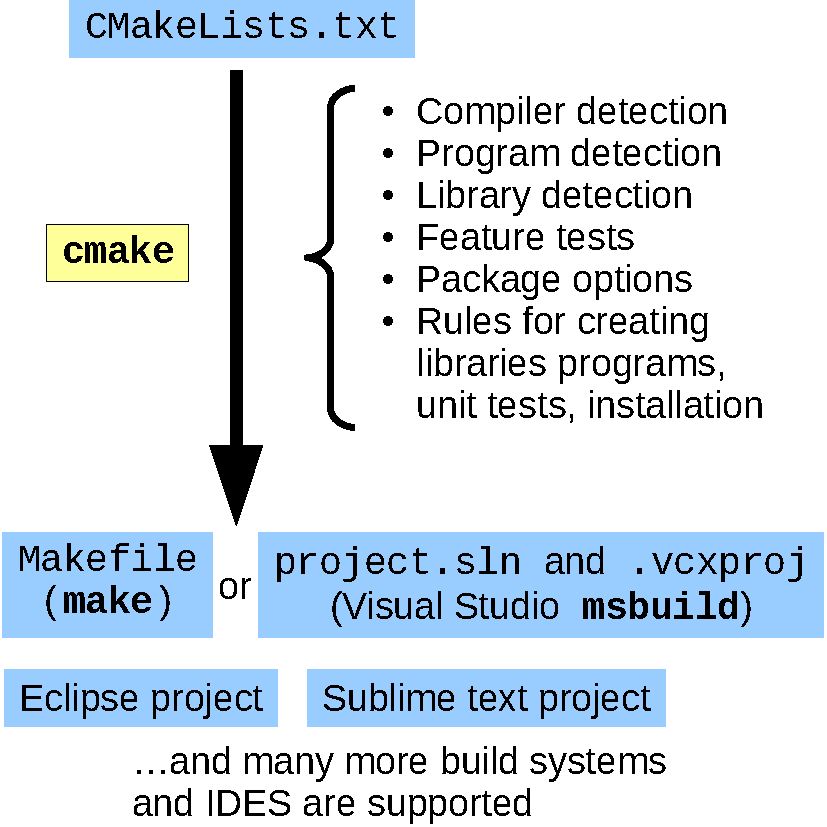
\includegraphics[width=0.65\textwidth]{cmake-flow}
\end{frame}

\begin{frame}
  \frametitle{\cmd{cmake} features}

  \begin{itemize}
  \item \cmd{cmake} is a generic cross-platform build system
  \item \cmd{cmake} generates build files for a large number of common
    build systems
  \item On FreeBSD, Linux and MacOS X, \cmd{make} \texttt{Makefile}s will be used
  \item On Windows with Visual Studio, \cmd{msbuild} \texttt{.sln}
    solution files will be used
  \item Eclipse, Sublime Text, Kate, Code::Blocks or several other
    IDEs or build systems may be used instead, if desired
  \end{itemize}
\end{frame}

\subsection{cmake demonstration}

\begin{frame}
  \frametitle{Using \cmd{cmake} (live demo)}
  \begin{block}{Basic cmake usage}
    \begin{itemize}
      \item Basic options
      \item Available generators
    \end{itemize}
  \end{block}
\end{frame}

\begin{frame}
  \frametitle{Using \cmd{cmake} (live demo)}
  \begin{block}{Building Bio-Formats on MacOS X}
    \begin{itemize}
      \item Running cmake
      \item Building
      \item Testing
      \item Installing
    \end{itemize}
  \end{block}
\end{frame}

\section{Using Bio-Formats}

\subsection{Downloading}

\begin{frame}
  \frametitle{Source and documentation downloads}
  \begin{itemize}
  \item \href{http://downloads.openmicroscopy.org/bio-formats-cpp/}{(Download source)}
  \item \href{http://www.openmicroscopy.org/site/support/bio-formats5.1/developers/index.html\#using-bio-formats-as-a-native-c-library}{(Documentation)}
  \item \href{http://www.openmicroscopy.org/site/support/bio-formats5.1/developers/cpp/tutorial.html}{(Tutorial)}
  \item \href{http://downloads.openmicroscopy.org/bio-formats-cpp/5.1.1/api/namespaces.html}{(Doxygen API reference)}
  \end{itemize}
\end{frame}

\subsection{Bio-Formats on Unix}

\begin{frame}[fragile]
  \frametitle{Building Bio-Formats on U\textsc{nix} (1)}
  \scriptsize
  Building from git or release zip:

  Configure the build:

  \begin{semiverbatim}
% mkdir /tmp/bfbuild
% cd /tmp/bfbuild
% /path/to/bioformats
\end{semiverbatim}

Run the build with either of:

  \begin{semiverbatim}
% make [VERBOSE=1]
% cmake --build .
\end{semiverbatim}
\end{frame}

\begin{frame}[fragile]
  \frametitle{Building Bio-Formats on U\textsc{nix} (2)}
  \scriptsize

Run the unit tests with any of:

  \begin{semiverbatim}
% make test
% cmake --build . --target test
% ctest [-V]
\end{semiverbatim}

Individual tests may be run by hand:

  \begin{semiverbatim}
% cpp/test/ome-bioformats/pixelbuffer
% cpp/test/ome-bioformats/pixelbuffer --gtest_help
\end{semiverbatim}

\begin{frame}[fragile]
  \frametitle{Building Bio-Formats on U\textsc{nix} (3)}
  \scriptsize

Install the build with either of:

  \begin{semiverbatim}
% make install [VERBOSE=1] [DESTDIR=/staging/path]
% cmake --build . --target install
\end{semiverbatim}

By default, this will install into \opt{CMAKE\_INSTALL\_PREFIX} which
will default to \path{/usr/local}.  Use \opt{DESTDIR} to install into
an alternative prefixed location, which is useful for testing and
packaging for release.
\end{frame}

\begin{frame}[fragile]
  \frametitle{Reading an OME-TIFF}
  \begin{lstlisting}
OMETIFFReader reader;

reader.setGroupFiles(true);
reader.setId(filename);
shared_ptr<MetadataStore> store = reader.getMetadataStore();

for (dimension_size_type series = 0U; series < reader.getSeriesCount(); ++series) {
  reader.setSeries(series);
  for (dimension_size_type plane = 0U; plane < reader.getPlaneCount(); ++plane) {
    VariantPixelBuffer pixels;
    reader.openBytes(plane, pixels);
  }
}
reader.close();
  \end{lstlisting}
\end{frame}

\begin{frame}[fragile]
  \frametitle{Writing an OME-TIFF}
  \begin{lstlisting}
shared_ptr<MetadataRetrieve> retrieve;
OMETIFFWriter writer;

writer.setMetadataRetrieve(retrieve);
writer.setInterleaved(interleaved);
writer.setId(filename);

for (dimension_size_type series = 0U; series < seriesCount; ++series) {
  writer.setSeries(series);
  for (dimension_size_type plane = 0U; plane < planeCount; ++plane) {
    VariantPixelBuffer pixels;
    writer.saveBytes(plane, pixels);
  }
}
writer.close();
  \end{lstlisting}
\end{frame}

\begin{frame}
  \frametitle{Tools for testing}
  \begin{block}{\cmd{bf-test}}
    \begin{itemize}
      \item \cmd{info}
      \item \cmd{view}
    \end{itemize}
  \end{block}
\end{frame}

\section{Future work}
\subsection{In progress}

\begin{frame}
  \frametitle{In the pipeline}
  \begin{itemize}
  \item \cmd{bfconvert}
  \item Units
  \item 2015-01 data model
  \item Windows support
  \item API improvements
  \end{itemize}
\end{frame}

\subsection{Feedback}
\begin{frame}
  \frametitle{Feedback}
  \begin{itemize}
  \item Which features do \emph{you} need
  \item Readers
  \item Writers
  \item Documenation
  \item Tools
  \item Support
  \item Integration
  \end{itemize}

  Any feedback would be welcome and will help set and prioritise the
  goals for future releases.
\end{frame}


\appendix

\section[]{Acknowledgements}

\frame{
  \frametitle{Acknowledgements}
  \parbox[t]{0.45\textwidth}{
    \begin{itemize}
    \item OME Team, Dundee
      \begin{itemize}
      \item Jason Swedlow
      \item Jean-Marie Burel
      \item Mark Carroll
      \item Andrew Patterson
      \item …and the rest of the team
      \end{itemize}
    \end{itemize}
  }
  \parbox[t]{0.45\textwidth}{
    \begin{itemize}
    \item Micron, Oxford
      \begin{itemize}
      \item Douglas Russell
      \end{itemize}
    \item Glencoe Software
      \begin{itemize}
      \item Melissa Linkert
      \item Josh Moore
      \end{itemize}
    \end{itemize}
  }

  \begin{center}
    \vcenteredhbox{
\includegraphics[width=0.25\textwidth]{ome}} \hfill
    \vcenteredhbox{
\includegraphics[width=0.2\textwidth]{dundee}}\hfill
    \vcenteredhbox{
\includegraphics[width=0.5\textwidth]{wellcome}}
  \end{center}
}

\end{document}
